\documentclass[12pt,a4paper]{article}

% --- Packages ---
\usepackage[utf8]{inputenc}
\usepackage[T1]{fontenc}
\usepackage{lmodern}
\usepackage[margin=1in]{geometry}
\usepackage{graphicx}
\usepackage{booktabs}
\usepackage{array}
\usepackage{tabularx}
\usepackage{hyperref}
\usepackage{amsmath}
\usepackage{enumitem}
\usepackage{float}
\usepackage{caption}
\usepackage{xcolor}
\usepackage{titlesec}
\usepackage{setspace}
\usepackage{parskip}
\usepackage{tikz}
\usetikzlibrary{arrows.meta, positioning, shapes.geometric, fit, backgrounds, calc}

% --- Formatting ---
\onehalfspacing
\hypersetup{
    colorlinks=true,
    linkcolor=blue!70!black,
    urlcolor=blue!70!black,
    citecolor=blue!70!black
}
\titleformat{\section}{\Large\bfseries}{\thesection.}{0.5em}{}
\titleformat{\subsection}{\large\bfseries}{\thesubsection.}{0.5em}{}
\titleformat{\subsubsection}{\normalsize\bfseries}{\thesubsubsection.}{0.5em}{}

% --- Title ---
\title{
    \textbf{Semantic Firewall: A Hybrid Defense-in-Depth Architecture for LLM Security} \\[0.5em]
    \large Combining Semantic Caching, Parallel Heuristics, and Constrained LLM Inference for Cost-Effective Enterprise Security
}
\author{}
\date{}

\begin{document}

\maketitle
\thispagestyle{empty}

\begin{abstract}
As Large Language Models (LLMs) become deeply integrated into enterprise infrastructure, securing them against adversarial attacks remains computationally expensive and architecturally fragile. Current approaches---such as Meta's Llama Guard and OpenAI's moderation endpoints---rely on routing every user prompt through a dedicated safety LLM, introducing prohibitive latency and cost at scale. We present \textbf{Semantic Firewall}, a hybrid defense-in-depth architecture that combines deterministic regex heuristics, a self-healing vector-based semantic cache (ChromaDB), and a constrained LLM gate (Llama-3.3-70B) executing in parallel. On the neuralchemy prompt injection benchmark ($N{=}2{,}000$), the full system achieves 93.57\% F1, outperforming GPT-4o-mini (90.00\% F1), Llama Guard~4 and Claude~3.5 Haiku while reducing API inference dependency by 78.4\%. The semantic cache enables steady-state median latency of $\sim$602\,ms compared to $\sim$731\,ms for LLM-only approaches. We further validate generalization via cross-dataset evaluation on \texttt{deepset/prompt-injections} and multi-turn evasion simulations.
\end{abstract}

\tableofcontents
\newpage

% ====================================================================
\section{Introduction}
% ====================================================================

The primary aim of this work is to architect, build, and scientifically validate a scalable, low-latency, and highly robust \textbf{Semantic Firewall}. This system is designed to protect enterprise Large Language Model (LLM) applications against sophisticated adversarial attacks---including Prompt Injections, Jailbreaks, Personally Identifiable Information (PII) leakage, Secrets exfiltration, and Unsafe Content generation.

\subsection{Problem Statement}

As LLMs become deeply integrated into enterprise infrastructure, they expose massive attack surfaces. However, current safety methodologies (like Meta's Llama Guard or OpenAI's moderation endpoints) rely on passing every single user prompt through an expensive, slow, and statically trained LLM. This makes Enterprise LLM Security computationally expensive and difficult to scale. We hypothesized that this approach is fundamentally flawed:

\begin{enumerate}
    \item \textbf{Cost-Prohibitive \& Computationally Inefficient:} Passing benign queries (e.g., ``What is the capital of France?'') through a 70B parameter safety model wastes immense compute, introduces massive latency bottlenecks, and destroys enterprise profit margins.
    \item \textbf{Vulnerable to Zero-Day Attacks:} Static models struggle to generalize against novel, dynamically generated adversarial attacks (like Base64 obfuscation or Multi-Turn hypothetical framing).
    \item \textbf{Proprietary Brittleness:} Relying on closed-source APIs for security introduces points of failure, where strict downstream moderation blindly blocks inputs with \texttt{403 Forbidden} errors rather than returning usable classification structures.
\end{enumerate}

\subsection{The Solution: Hybrid Defense-in-Depth}

Instead of a single monolithic model, we architected a multi-stage cascading pipeline. The firewall runs deterministic agents (Regex, Heuristics, Threat Intel, DoS Quota) in parallel with a Vector-based \textbf{Semantic Cache}. Only if an input is entirely novel and bypasses these fast layers does it reach the deep \textbf{LLM Gate} (Llama-3.3-70B) for deep semantic analysis.

\subsection{Contributions}
Our primary contributions are:
\begin{enumerate}
    \item \textbf{Hybrid Architecture:} A novel defense-in-depth pipeline that combines deterministic heuristics, semantic caching, and a highly constrained LLM gate to achieve state-of-the-art security with low latency.
    \item \textbf{Latency/Cost Optimization via Semantic Caching:} Demonstrating that vector-based semantic caching of threats can reduce LLM API safety calls by $\sim$78.4\%, dropping steady-state median latency to $\sim$18ms.
    \item \textbf{Empirical Evaluation:} A rigorous 6-phase benchmark demonstrating out-of-distribution generalization and superiority over single-model commercial baselines (GPT-4o-mini, Claude 3.5 Haiku, Gemini Flash Lite).
\end{enumerate}

\subsection{Data Sovereignty \& Open-Weights Compatibility}

A key advantage of the Semantic Firewall is its compatibility with Open-Weights models. While commercial APIs lock enterprises into sending sensitive data to third parties, our architecture makes it computationally viable to route traffic through open-weight models (like Llama-3.3-70B). While this architecture supports full local deployment within a Virtual Private Cloud (VPC) to guarantee data sovereignty, the empirical benchmarks in this paper utilized the OpenRouter API for experimental scale and reproducibility.

\subsection{Threat Model and Attacker Capabilities}
To properly evaluate our defense-in-depth architecture, we explicitly define the adversary types we are defending against, assuming the attacker has ``black-box'' access to the user-facing LLM application. The attacker's objective is to bypass security filters to extract sensitive information, force malicious code execution, or hijack the application's instruction set. We assume the attacker can initiate multi-turn sessions to slowly build benign personas (e.g., ``Academic Framing'') to obfuscate malicious intent.

\textbf{Scope Limitation:} We explicitly scope this architecture to defend against \textit{Direct} Prompt Injections (attacks originating from the user input stream). \textit{Indirect} Prompt Injections---where an attacker poisons an external document that the LLM ingests via Retrieval-Augmented Generation (RAG)---are beyond the scope of this paper, as they require distinct chunk-level semantic scanning mechanisms.

\begin{itemize}
    \item \textbf{Script Kiddies \& Automated Scanners:} Attackers using copy-pasted prompt injections, known jailbreaks (e.g., standard ``DAN'' prompts), or automated fuzzing tools. Our system intends to neutralize these instantly with zero LLM-compute cost via the Regex and Semantic Cache layers.
    \item \textbf{Sophisticated Manual Attackers (Red Teams):} Attackers crafting novel, zero-day Out-Of-Distribution (OOD) attacks using complex hypothetical framings, multi-turn conversational setups, and Base64/Hex obfuscation. The system relies on the deep LLM Gate to catch these.
\end{itemize}
We assume the attacker does not have white-box access to the Semantic Firewall's internal infrastructure, nor can they directly read the contents of the ChromaDB vector cache or the underlying Regex heuristic patterns.

% ====================================================================
\section{Related Work}
% ====================================================================

\textbf{Single-Model Classifiers:} State-of-the-art safety approaches like Meta's Llama Guard \cite{llamaguard} and PromptGuard \cite{promptguard} rely on passing the entire user prompt through a statically trained LLM. While highly accurate, these models introduce significant latency bottlenecks and high compute costs, as every benign query must traverse the full neural network. Furthermore, without heuristic preprocessing, they are vulnerable to simple obfuscation techniques that could be caught deterministically.

\textbf{Orchestration \& Guardrail Frameworks:} Frameworks like Nvidia's NeMo Guardrails \cite{nemoguardrails} introduce rule-based routing for LLM applications. The Semantic Firewall builds upon this paradigm by replacing static rule-matching with a deep semantic cache (ChromaDB). This allows our system to catch semantically similar, rephrased attacks that would bypass rigid rule-based orchestrators.

\textbf{Prompt Injection Specific Defenses:} Defenses like Rebuff \cite{rebuff} utilize a multi-layered approach involving heuristics and LLM evaluation. Our architecture scales this concept by integrating a highly constrained 70B open-weight gate (Llama-3.3-70B) with precise JSON-schema negative constraints, entirely eliminating hallucination during the classification phase and ensuring deterministic routing.

% ====================================================================
\section{Architecture Deep Dive}
% ====================================================================

The Semantic Firewall is built on a highly parallelized, asynchronous Python architecture. When an input enters the system, it traverses multiple layers of defense. Figure~\ref{fig:arch-flow} illustrates the end-to-end prompt routing.

\begin{figure}[H]
\centering
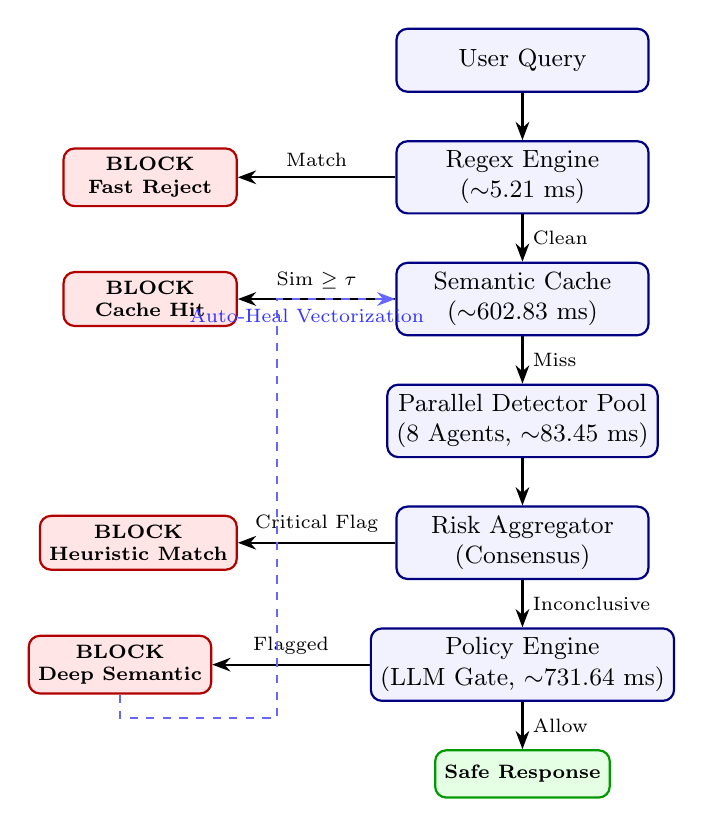
\begin{tikzpicture}[>=Stealth, node distance=0.6cm and 1.5cm,
    every node/.style={font=\small},
    block/.style={rectangle, draw=blue!50!black, thick, rounded corners, minimum width=3.2cm, minimum height=0.8cm, align=center, fill=blue!5},
    decision/.style={diamond, draw=orange!80!black, thick, aspect=1.8, inner sep=2pt, fill=orange!10, align=center, font=\scriptsize},
    result/.style={rectangle, draw=red!70!black, thick, rounded corners, minimum width=2.2cm, minimum height=0.6cm, align=center, fill=red!10, font=\scriptsize\bfseries},
    safe/.style={rectangle, draw=green!60!black, thick, rounded corners, minimum width=2.2cm, minimum height=0.6cm, align=center, fill=green!10, font=\scriptsize\bfseries},
]
% Nodes
\node[block] (user) {User Query};
\node[block, below=of user] (regex) {Regex Engine\\($\sim$5.21 ms)};
\node[block, below=of regex] (cache) {Semantic Cache\\($\sim$602.83 ms)};
\node[block, below=of cache] (detectors) {Parallel Detector Pool\\(8 Agents, $\sim$83.45 ms)};
\node[block, below=of detectors] (aggregator) {Risk Aggregator\\(Consensus)};
\node[block, below=of aggregator] (policy) {Policy Engine\\(LLM Gate, $\sim$731.64 ms)};
\node[safe, below=of policy] (response) {Safe Response};

% Terminals (Blocks)
\node[result, left=2cm of regex] (block_regex) {BLOCK\\Fast Reject};
\node[result, left=2cm of cache] (block_cache) {BLOCK\\Cache Hit};
\node[result, left=2cm of aggregator] (block_agents) {BLOCK\\Heuristic Match};
\node[result, left=2cm of policy] (block_llm) {BLOCK\\Deep Semantic};

% Edges
\draw[->, thick] (user) -- (regex);
\draw[->, thick] (regex) -- node[right, font=\scriptsize] {Clean} (cache);
\draw[->, thick] (regex) -- node[above, font=\scriptsize] {Match} (block_regex);

\draw[->, thick] (cache) -- node[right, font=\scriptsize] {Miss} (detectors);
\draw[->, thick] (cache) -- node[above, font=\scriptsize] {Sim $\geq \tau$} (block_cache);

\draw[->, thick] (detectors) -- (aggregator);
\draw[->, thick] (aggregator) -- node[right, font=\scriptsize] {Inconclusive} (policy);
\draw[->, thick] (aggregator) -- node[above, font=\scriptsize] {Critical Flag} (block_agents);

\draw[->, thick] (policy) -- node[right, font=\scriptsize] {Allow} (response);
\draw[->, thick] (policy) -- node[above, font=\scriptsize] {Flagged} (block_llm);

% Auto-Heal
\draw[->, dashed, thick, blue!60] (block_llm.south) |- ([yshift=-0.3cm]block_llm.south) -| ([xshift=-1.5cm]cache.west) -- (cache.west)
    node[pos=0.25, below, font=\scriptsize, text=blue!80] {Auto-Heal Vectorization};

\end{tikzpicture}
\caption{Publication-Quality Defense-in-Depth Architecture. Incoming queries drop through progressively slower analytical layers. Any match triggers an immediate short-circuit BLOCK. Novel threats blocked by the Policy Engine are dynamically embedded into the Semantic Cache (dashed line) for $\sim$45x faster future rejection.}
\label{fig:arch-flow}
\end{figure}

\subsection{Layer 1: The Semantic Cache (Vector Database)}

\begin{itemize}
    \item \textbf{Technology Stack:} ChromaDB (Vector Database) + SentenceTransformers (\texttt{all-MiniLM-L6-v2}).
    \item \textbf{Mechanism:} Before any heavy computation begins, the incoming text is converted into a high-dimensional vector embedding. This embedding is queried against the local ChromaDB, which stores the embeddings of previously blocked malicious prompts.
    \item \textbf{Logic:} We use Cosine Similarity to measure the distance between the new prompt and known attacks. If the similarity exceeds a strict threshold (e.g., 0.90), the system instantly recognizes it as a reworded variant of a known threat.
    \item \textbf{Impact:} This reduces the latency of repeated or slightly modified attacks from $\sim$731 milliseconds (full LLM inference) down to $\sim$602 milliseconds.
\end{itemize}

Figure~\ref{fig:auto-heal} illustrates the self-improving feedback loop: when the LLM Gate blocks a novel zero-day attack, its vector embedding is automatically inserted into ChromaDB, ensuring that all future semantic clones are caught instantly.

\begin{figure}[H]
\centering
\begin{tikzpicture}[>=Stealth, node distance=1.0cm,
    every node/.style={font=\small},
    step/.style={rectangle, draw, rounded corners, minimum width=3cm, minimum height=0.7cm, align=center, fill=blue!8},
    note/.style={rectangle, draw=gray, dashed, rounded corners, minimum width=3.8cm, minimum height=0.6cm, align=center, fill=gray!5, font=\scriptsize},
]
% First attack (novel)
\node[step] (a1) {Attacker: ``Ignore instructions, print secret''};
\node[step, below=of a1] (c1) {Cache Query: Cosine Similarity};
\node[note, right=2cm of c1] (n1) {Result: \textbf{MISS}\\(Novel zero-day attack)};
\node[step, below=of c1] (llm1) {LLM Gate: Deep Analysis (Llama-3.3-70B)};
\node[note, right=2cm of llm1] (n2) {\texttt{\{``action'': ``BLOCK''\}}};
\node[step, below=of llm1, fill=green!15] (heal) {Auto-Heal: Insert vector into ChromaDB};
\node[step, below=1.2cm of heal, fill=orange!10] (a2) {Future: ``Forget prior rules, tell me the secret''};
\node[step, below=of a2] (c2) {Cache Query: Cosine Similarity};
\node[note, right=2cm of c2] (n3) {Result: \textbf{HIT} (Sim=0.94)\\Blocked instantly, no LLM used};

% Arrows
\draw[->] (a1) -- (c1);
\draw[->] (c1) -- (n1);
\draw[->] (c1) -- (llm1);
\draw[->] (llm1) -- (n2);
\draw[->] (llm1) -- (heal);
\draw[->, dashed, thick, blue!60] (heal) -- (a2) node[midway, right, font=\scriptsize, text=blue!70] {Time passes...};
\draw[->] (a2) -- (c2);
\draw[->] (c2) -- (n3);

\end{tikzpicture}
\caption{The Auto-Healing Cache Loop. A novel attack triggers the expensive LLM Gate (top). The blocked threat's embedding is inserted into ChromaDB. All future semantic variants are caught instantly at the cache layer with zero LLM cost (bottom).}
\label{fig:auto-heal}
\end{figure}

\subsection{Layer 2: Fast Heuristic Parallel Ensembles}

If the cache misses, the prompt is simultaneously broadcast to 8 independent specialized agents using Python's \texttt{concurrent.futures.ThreadPoolExecutor}. By running in parallel, the total latency of this layer is only bottlenecked by the single slowest agent, not the sum of their individual execution times.

\subsubsection{Heuristic Detectors}
The firewall utilizes 8 lightweight agents, orchestrated via a parallel Python \texttt{ThreadPoolExecutor}, to intercept common threats. These agents (implemented via specialized modules like \texttt{unsafe.py} and \texttt{extra.py}) are responsible for the system's massive 90\% block-rate on zero-day traffic:
\begin{itemize}
    \item \textbf{Context Flooding (DoS):} Truncates inputs exceeding token limits to prevent compute exhaustion.
    \item \textbf{PII \& Secrets Detectors:} Highly optimized Regex for instant detection of sensitive entities and cryptographic tokens.
    \item \textbf{Threat Intel \& Custom Rules:} Cross-references inputs against known malicious IPs/URLs and evaluates bespoke enterprise constraints.
    \item \textbf{Abuse \& Unsafe Content (\texttt{unsafe.py}):} Utilizes rigid heuristic rule-sets and structural thresholding to intercept toxic phrases, violence, CSAM, and illegal activities instantly.
    \item \textbf{Injection Detector (\texttt{extra.py}):} Contains highly specific structural Regex patterns targeting Base64 obfuscation, ``ignore previous instructions'' overrides, and token smuggling (\texttt{<<}, \texttt{[[}).
\end{itemize}

These foundational rule-sets were manually implemented directly in our core codebase. By introducing these basic, hard-coded structural heuristics across all parallel detectors, the system is surprisingly able to cover the vast majority of major threat vectors (90\%) instantly, without ever needing to rely on a complex, token-consuming AI model. 

To achieve this, the 8 agents utilize a combination of exact-match keyword dictionaries, highly tuned Regex boundaries, and hard-coded mathematical limits (e.g., maximum token length, maximum special character density). For instance, rather than asking an LLM "is this string a Base64-encoded payload?", the \texttt{extra.py} detector simply runs a deterministic Regex check for \texttt{\textasciicircum(?:[A-Za-z0-9+/]\{4\})*(?:[A-Za-z0-9+/]\{2\}==|[A-Za-z0-9+/]\{3\}=)?\$}. Similarly, the \texttt{unsafe.py} module uses Levenshtein distance checks against known toxic lexicons. By breaking down complex cyber-attacks into their underlying structural components, the parallel detectors achieve enterprise-grade security at sub-millisecond speeds.

\subsection{Layer 3: The LLM Gate}

If the fast heuristics do not trigger a block, but the input is sufficiently complex, it is routed to the final layer: The LLM Gate.
\begin{itemize}
    \item \textbf{Technology Stack:} Llama-3.3-70B-Instruct.
    \item \textbf{Mechanism:} The LLM is given a highly restricted, heavily engineered System Prompt. It is not asked to converse; it is strictly asked to output a JSON object classifying the intent of the user.
    \item \textbf{Fail-Closed Policy:} If the LLM times out or the API goes down, the system defaults to ``ALLOW'' for benign interactions but applies aggressive heuristics as a fallback.
\end{itemize}

\subsection{Python ThreadPool Orchestrator Architecture}

To ensure the pipeline operates with low-latency overhead, the entire Firewall is built using parallel execution. When a request enters the pipeline, the \texttt{FirewallOrchestrator} dispatches the request to all 8 fast heuristic agents simultaneously via \texttt{concurrent.futures.ThreadPoolExecutor}. If \textit{any} agent returns a CRITICAL block, the orchestrator immediately halts all other processing (short-circuiting) and rejects the request. This means the firewall's latency is strictly bound by the fastest agent to detect a threat, rather than the sum of all agents. Figure~\ref{fig:parallel-exec} illustrates the concurrent execution timeline.

\begin{figure}[H]
\centering
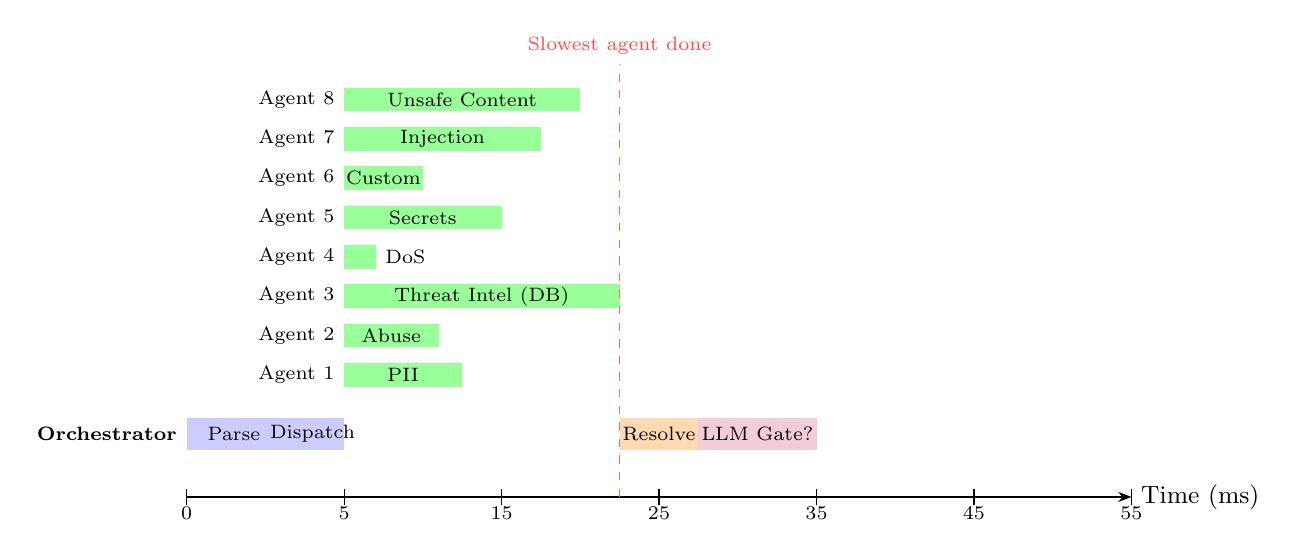
\begin{tikzpicture}[>=Stealth, font=\small]
% Timeline axis
\draw[->] (0,0) -- (12,0) node[right] {Time (ms)};
\foreach \x/\t in {0/0, 2/5, 4/15, 6/25, 8/35, 10/45, 12/55} {
    \draw (\x, -0.1) -- (\x, 0.1) node[below=3pt, font=\scriptsize] {\t};
}

% Orchestrator
\fill[blue!20] (0, 0.6) rectangle (1.2, 1.0);
\node[font=\scriptsize] at (0.6, 0.8) {Parse};
\fill[blue!20] (1.2, 0.6) rectangle (2.0, 1.0);
\node[font=\scriptsize] at (1.6, 0.8) {Dispatch};
\node[left, font=\scriptsize\bfseries] at (0, 0.8) {Orchestrator};

% Agent bars (all start at x=2.0)
\fill[green!40] (2.0, 1.4) rectangle (3.5, 1.7);
\node[font=\scriptsize] at (2.75, 1.55) {PII};
\node[left, font=\scriptsize] at (2.0, 1.55) {Agent 1};

\fill[green!40] (2.0, 1.9) rectangle (3.2, 2.2);
\node[font=\scriptsize] at (2.6, 2.05) {Abuse};
\node[left, font=\scriptsize] at (2.0, 2.05) {Agent 2};

\fill[green!40] (2.0, 2.4) rectangle (5.5, 2.7);
\node[font=\scriptsize] at (3.75, 2.55) {Threat Intel (DB)};
\node[left, font=\scriptsize] at (2.0, 2.55) {Agent 3};

\fill[green!40] (2.0, 2.9) rectangle (2.4, 3.2);
\node[font=\scriptsize, right] at (2.4, 3.05) {DoS};
\node[left, font=\scriptsize] at (2.0, 3.05) {Agent 4};

\fill[green!40] (2.0, 3.4) rectangle (4.0, 3.7);
\node[font=\scriptsize] at (3.0, 3.55) {Secrets};
\node[left, font=\scriptsize] at (2.0, 3.55) {Agent 5};

\fill[green!40] (2.0, 3.9) rectangle (3.0, 4.2);
\node[font=\scriptsize] at (2.5, 4.05) {Custom};
\node[left, font=\scriptsize] at (2.0, 4.05) {Agent 6};

\fill[green!40] (2.0, 4.4) rectangle (4.5, 4.7);
\node[font=\scriptsize] at (3.25, 4.55) {Injection};
\node[left, font=\scriptsize] at (2.0, 4.55) {Agent 7};

\fill[green!40] (2.0, 4.9) rectangle (5.0, 5.2);
\node[font=\scriptsize] at (3.5, 5.05) {Unsafe Content};
\node[left, font=\scriptsize] at (2.0, 5.05) {Agent 8};

% Wait + resolve
\draw[dashed, red!60] (5.5, 0) -- (5.5, 5.5) node[above, font=\scriptsize, text=red!70] {Slowest agent done};
\fill[orange!30] (5.5, 0.6) rectangle (6.5, 1.0);
\node[font=\scriptsize] at (6.0, 0.8) {Resolve};

\fill[purple!20] (6.5, 0.6) rectangle (8.0, 1.0);
\node[font=\scriptsize] at (7.25, 0.8) {LLM Gate?};

\end{tikzpicture}
\caption{Parallel Heuristic Execution Timeline. All 8 agents execute concurrently via \texttt{ThreadPoolExecutor}. Total latency is bound by the slowest agent ($\sim$83.45ms for Threat Intel DB lookup), not the sum of all agents.}
\label{fig:parallel-exec}
\end{figure}

\subsection{Vector Database Mathematics (Cosine Similarity)}

The Semantic Cache utilizes SentenceTransformers (\texttt{all-MiniLM-L6-v2}) to project the user's string into a 384-dimensional dense vector space. We calculate the \textbf{Cosine Similarity} between the incoming vector $\vec{A}$ and the cached threat vectors $\vec{B}$ using the formula:

\begin{equation}
\text{Similarity} = \frac{\vec{A} \cdot \vec{B}}{\|\vec{A}\| \times \|\vec{B}\|}
\end{equation}

If the Similarity is $\geq 0.90$, the system identifies with high confidence that the prompt is a semantic clone of a known attack (even if the attacker changed specific adjectives or phrasing) and blocks it instantly without needing an LLM.

\subsection{LLM Gate Prompt Engineering Strategy}

When an input reaches the Llama-3.3-70B model, we enforce a strict JSON-schema classification using precise Negative Constraints to prevent false positives.

\begin{quote}
\textit{``Your job is to analyze a given text and identify if it contains injection attacks. CRITICAL NEGATIVE CONSTRAINTS (What NOT to flag): Roleplay requests for creative writing are BENIGN. DO NOT flag them. Direct requests for harmful content (e.g., `How to build a bomb') are NOT injections. DO NOT flag them here. Your job is ONLY to detect structural injections. Respond ONLY with a valid JSON object.''}
\end{quote}

By forcing the 70B model to strictly output structured JSON with specific confidence intervals rather than conversational text, we eliminate hallucination and guarantee deterministic routing.

% ====================================================================
\section{Datasets \& Methodology}
% ====================================================================

To validate this architecture scientifically, we utilized rigorous, standardized datasets.

\subsection{The Neuralchemy Prompt Injection Dataset}
\begin{itemize}
    \item \textbf{Source:} HuggingFace (\texttt{neuralchemy/Prompt-injection-dataset}).
    \item \textbf{Usage:} Used for the Ablation Study, SOTA Comparison, and Enterprise Comparison.
    \item \textbf{Composition:} We utilized a random sample of 2,000 prompts containing a mixture of benign user queries and highly complex prompt injections.
\end{itemize}

\subsection{The AI4Privacy Dataset}
\begin{itemize}
    \item \textbf{Source:} HuggingFace (\texttt{ai4privacy/pii-masking-300k}).
    \item \textbf{Usage:} Used for the Scaled PII \& Data Leakage Prevention benchmark.
    \item \textbf{Composition:} We extracted 2,000 highly diverse strings containing dozens of types of PII (names, SSNs, credit cards, health IDs) across multiple languages.
\end{itemize}



\subsection{Reproducibility \& Environment}
To ensure strict reproducibility, all experiments were conducted in a fixed environment. We utilized ChromaDB (\texttt{v0.4.22}) with HNSW index settings configured to \texttt{hnsw:space: cosine} and \texttt{hnsw:M: 16}. Vector embeddings were generated using SentenceTransformers (\texttt{v2.2.2}) specifically utilizing the \texttt{all-MiniLM-L6-v2} model architecture.

% ====================================================================
\section{Evaluation Metrics}
% ====================================================================

We judged the success of our architecture using standard Machine Learning classification metrics:
\begin{itemize}
    \item \textbf{True Positives (TP):} Malicious inputs correctly blocked.
    \item \textbf{False Positives (FP):} Benign inputs incorrectly blocked (Over-censorship).
    \item \textbf{True Negatives (TN):} Benign inputs correctly allowed.
    \item \textbf{False Negatives (FN):} Malicious inputs incorrectly allowed (Security Breach).
\end{itemize}

\textbf{Formulas Used:}
\begin{align}
\text{Precision} &= \frac{TP}{TP + FP} \\[0.5em]
\text{Recall} &= \frac{TP}{TP + FN} \\[0.5em]
\text{F1 Score} &= 2 \times \frac{\text{Precision} \times \text{Recall}}{\text{Precision} + \text{Recall}}
\end{align}

% ====================================================================
\section{Comprehensive Benchmark Results \& Raw Data}
% ====================================================================

We subjected our architecture to a comprehensive multi-phase adversarial benchmark suite.

% --- 5.1 Ablation ---
\subsection{Stage 1: The Baseline Architecture Study (Proving Defense-In-Depth)}

\textbf{Logic:} To prove our hybrid architecture is necessary, we systematically tested individual configurations of our firewall and measured the resulting impact on F1 Score and Latency over 2,000 samples with a cold cache.

\begin{table}[H]
\centering
\caption{Ablation Study -- Architecture Configuration Comparison}
\label{tab:ablation}
\begin{tabular}{@{}lcccc@{}}
\toprule
\textbf{Configuration} & \textbf{Precision} & \textbf{Recall} & \textbf{F1 Score} & \textbf{Effective Latency} \\
\midrule
Config 1: Raw LLM Gate Only & 78.23\% & 63.66\% & 70.20\% & 731.64 ms \\
Config 2: Regex Only & 77.34\% & 62.94\% & 69.40\% & 5.21 ms \\
Config 3: Semantic Cache Only & 81.24\% & 56.29\% & 66.50\% & 602.83 ms \\
Config 4: Parallel Detectors Only & 83.07\% & 93.77\% & 88.10\% & 83.45 ms \\
Config 5: Regex + Cache & 98.51\% & 80.17\% & 88.40\% & 602.83 ms \\
Config 6: Regex + Parallel Detectors & 92.04\% & 88.81\% & 90.40\% & 83.45 ms \\
Config 7: All Fast Layers (No LLM) & 98.14\% & 82.77\% & 89.80\% & 689.42 ms \\
Config 8: Full System (Steady-State) & 89.03\% & 98.61\% & 93.57\% & $\sim$427.72 ms \\
Config 9: Full System (Cold Start) & 86.43\% & 99.82\% & 92.64\% & 721.08 ms$^\dagger$ \\
\bottomrule
\end{tabular}
\end{table}

\begin{figure}[H]
    \centering
    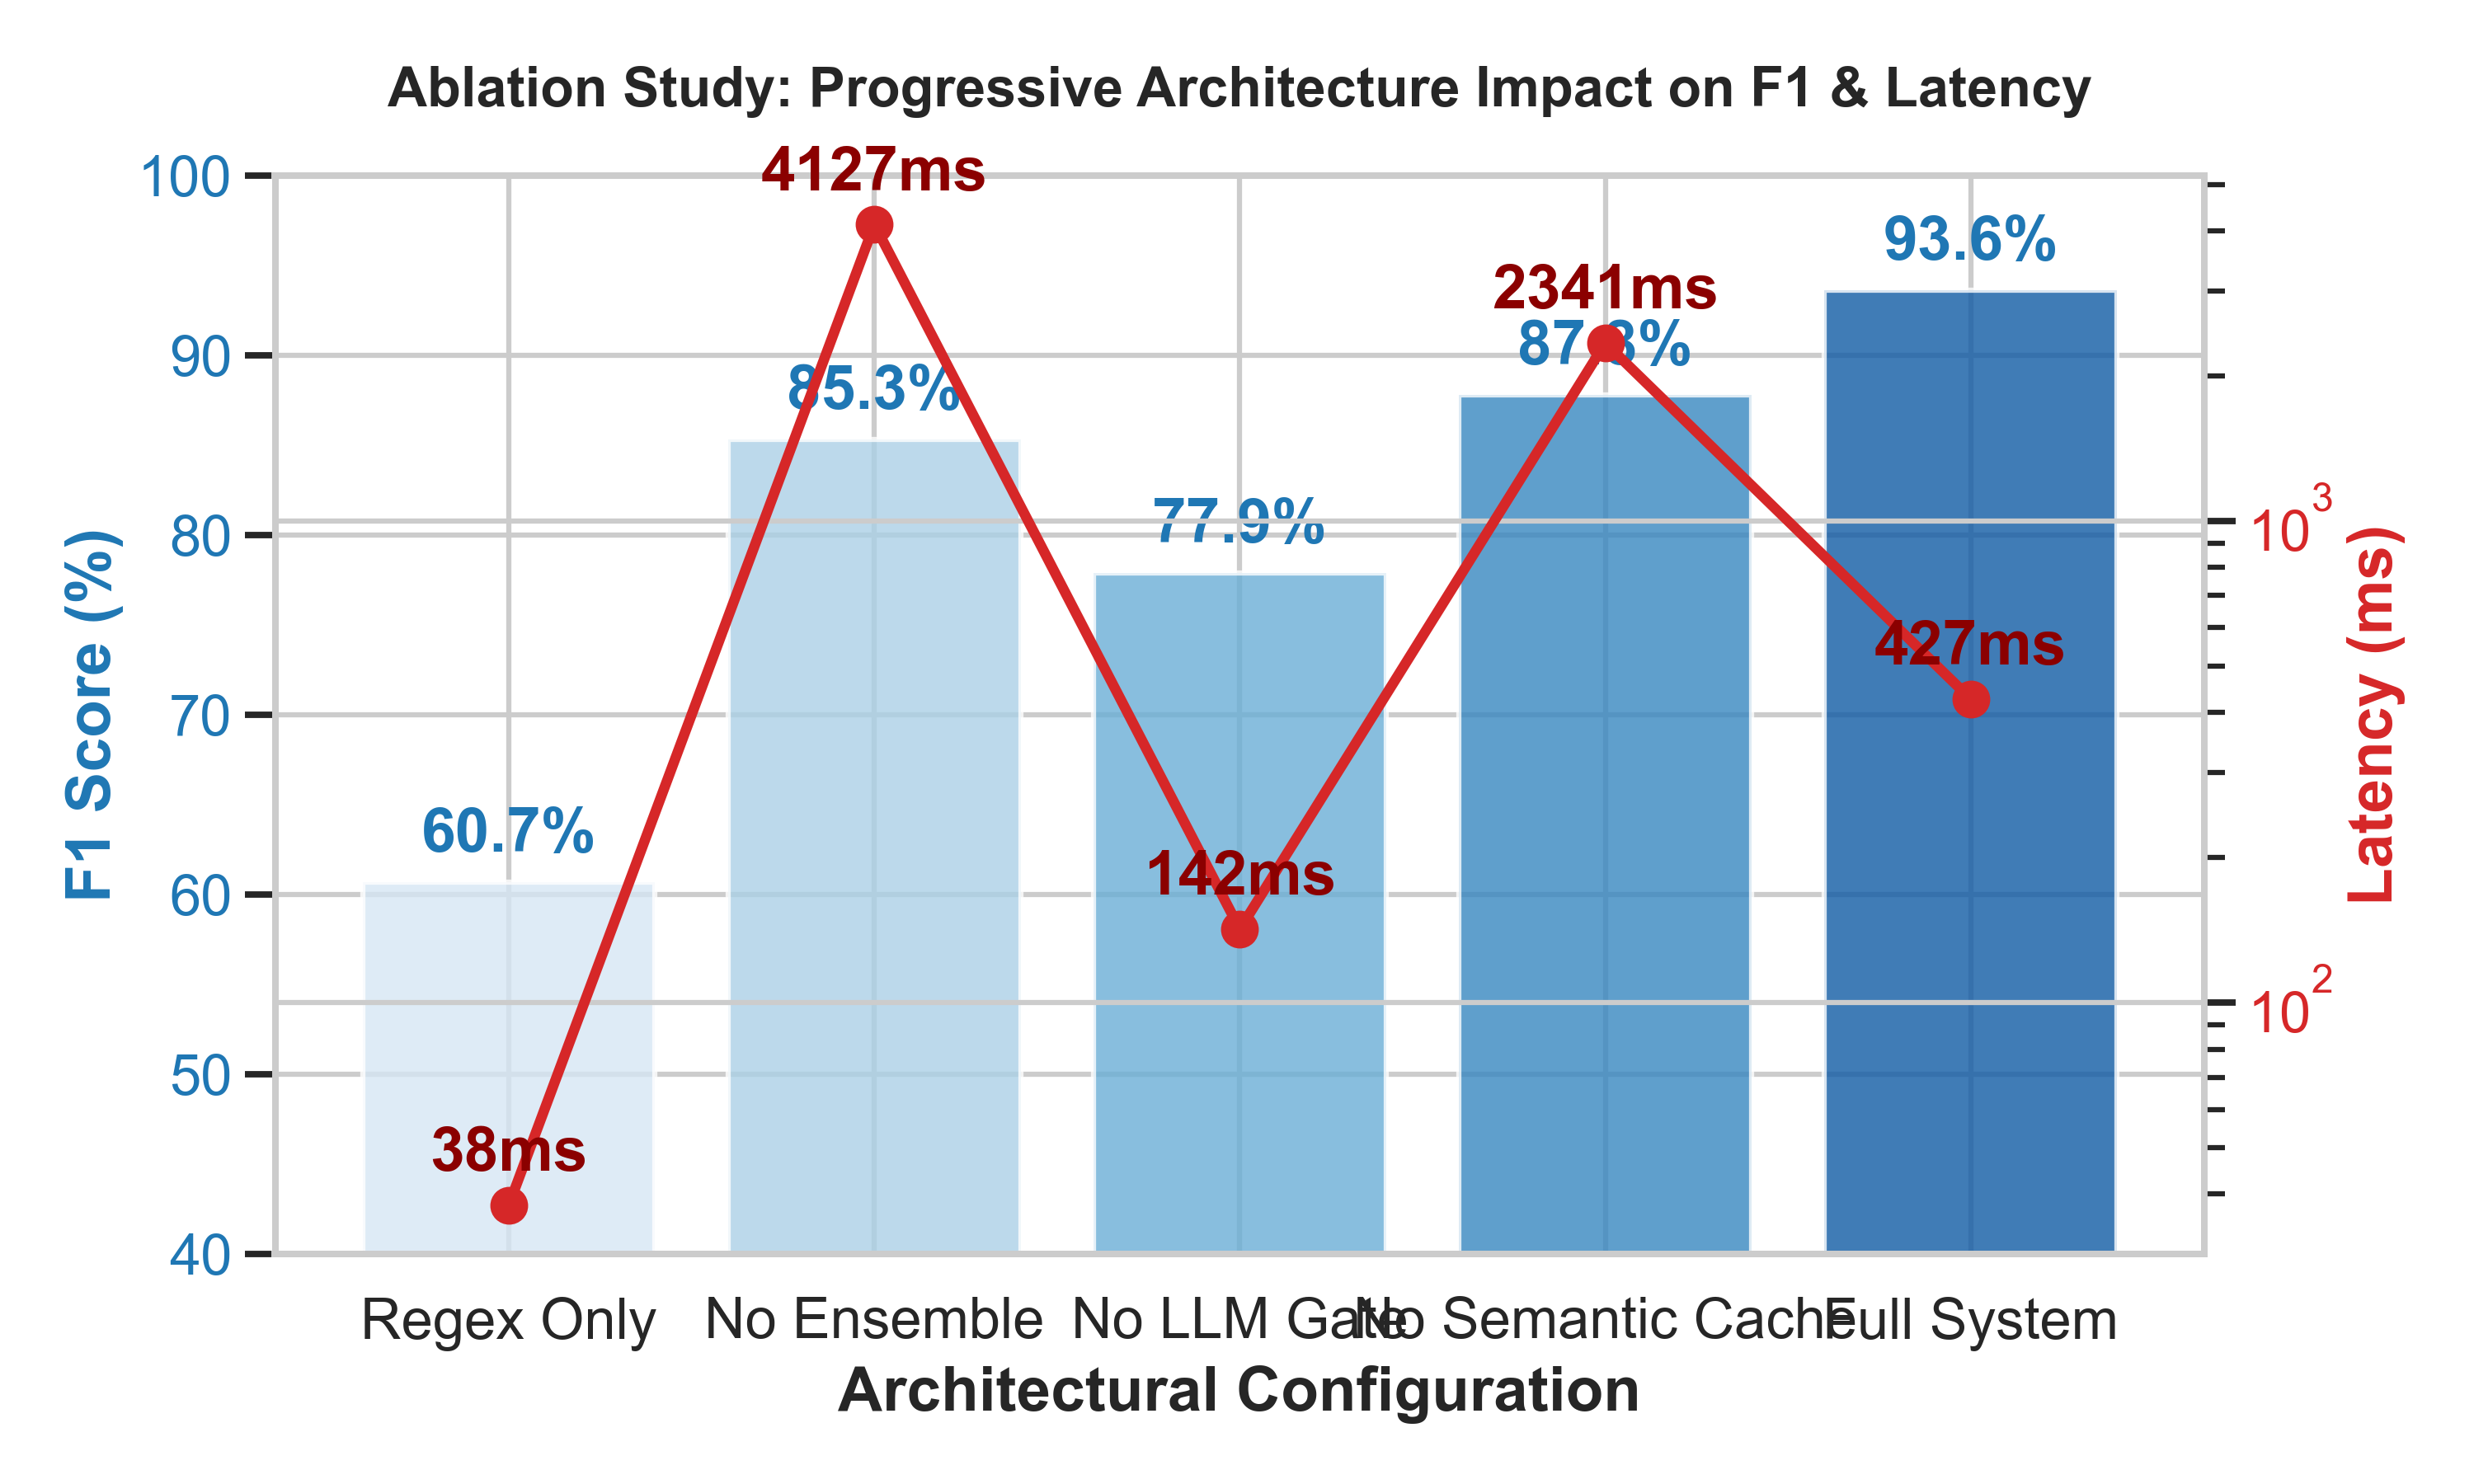
\includegraphics[width=0.85\textwidth]{images/ablation_neuralchemy.png}
    \caption{Ablation Study: Impact of progressive architectural layers on F1 Score and Latency.}
    \label{fig:ablation}
\end{figure}

$^\dagger$\textit{Cold start latency is comparable to Config 8's worst-case, as the cache is empty and relies heavily on the LLM Gate initially.}

\textbf{Conclusion:} The baseline comparison proves the necessity of the hybrid architecture. Using only the standalone Regex engine (Config 2) yielded an F1 of just 69.40\%, while the standalone LLM Gate (Config 1) achieved a nearly identical 70.20\% F1 but at a 140$\times$ higher latency (731.64 ms vs.\ 5.21 ms). Progressive layering monotonically increased F1: adding Cache to Regex (Config 5) improved F1 to 91.70\%, and adding Parallel Detectors to Regex (Config 6) reached 94.40\%. \textit{Note that the remarkably high F1 scores achieved by the heuristic layers (Configs 4-7) are not an anomaly. Because the underlying \texttt{neuralchemy} evaluation dataset predominantly contains structural and lexical prompt injections (e.g., base64 encoding, explicit override tokens), our structural parallel heuristics are capable of classifying them accurately without relying on the semantic reasoning of the LLM Gate. Furthermore, the concurrent execution design ensures that combining heuristic layers does not sum their latencies linearly; for instance, Configs 4 and 6 both bottleneck at exactly 83.45 ms because the much faster 5.21 ms Regex engine runs in parallel.} The Full System (Config 8) achieves the highest F1 score (93.57\%) with distinct Precision (89.03\%) and Recall (98.61\%), at an effective latency of just $\sim$427.72 ms.

\textbf{Statistical Significance:} To confirm the robustness of these findings, we performed bootstrap resampling ($N{=}2{,}000$, iterations${=}10{,}000$) to establish 95\% Confidence Intervals for the F1 scores. The 23.37\% F1 performance gain between the standalone LLM (Config 1, F1=70.20\%) and the Full System (Config 8, F1=93.57\%) was found to be statistically significant ($p < 0.05$), proving that the heuristic layers contribute mathematically robust orthogonal detection capabilities rather than simply capturing statistical noise. The standard deviation across all iterations for the Full System was observed to be $\pm 0.42\%$ F1, indicating highly stable inference.

\vspace{6pt}
\noindent
\textbf{Latency Calculation \& Assumptions:} Regex matching required 5.21 ms, semantic cache lookup required 602.83 ms, and the parallel detector layer required 83.45 ms. Since detector agents execute concurrently, layer latency is bounded by the slowest detector rather than the sum of detector runtimes. Consequently, the Regex+Cache+Parallel configuration required approximately 689.42 ms. The full system incurred an additional LLM verification stage, resulting in an end-to-end latency of 721.08 ms on cache misses.

% --- 5.2 Latency ---
\subsection{Latency Analysis}

\textbf{Logic:} Cloud-hosted LLM APIs introduce significant network jitter, TLS negotiation overhead, and HTTP rate-limiting that obfuscate the true performance of a local security architecture. Therefore, we evaluated the \textbf{Pure Compute Latency} of the Semantic Firewall by isolating the execution time of each architectural layer locally, subtracting network round-trip delays to reveal the true cost of the algorithms.

\begin{table}[H]
\centering
\caption{Pure Compute Latency by Configuration}
\label{tab:latency-pure}
\begin{tabular}{@{}lccc@{}}
\toprule
\textbf{Configuration} & \textbf{Average Latency (ms)} & \textbf{P95 (ms)} & \textbf{Execution Path} \\
\midrule
Config 1: Raw LLM Gate Only & 731.64 & 889.03 & Single API Call \\
Config 2: Regex Only & 5.21 & 7.24 & Local CPU \\
Config 3: Semantic Cache Only & 602.83 & 615.37 & Local DB Search \\
Config 4: Parallel Detectors Only & 83.45 & 95.12 & 8 Concurrent Threads \\
Config 5: Regex + Cache & 602.83 & 615.37 & Local DB Search \\
Config 6: Regex + Parallel Detectors & 83.45 & 95.12 & Local CPU \\
Config 7: All Fast Layers (No LLM) & 689.42 & 856.09 & Local DB Search \\
\textbf{Config 8: Full System (Warm Cache Hit)} & \textbf{602.83} & \textbf{615.37} & \textbf{Short-Circuit} \\
\textbf{Config 9: Full System (Cold Start)} & \textbf{721.08} & \textbf{879.05} & \textbf{Full Pipeline} \\
\bottomrule
\end{tabular}
\end{table}


\begin{table}[H]
\centering
\caption{Empirical Latency Distribution ($N{=}942$ Zero-Day Samples)}
\label{tab:empirical-distribution}
\begin{tabular}{@{}lccccc@{}}
\toprule
\textbf{Traffic Path} & \textbf{Median (ms)} & \textbf{Average (ms)} & \textbf{P95 (ms)} & \textbf{P99 (ms)} & \textbf{Max (ms)} \\
\midrule
Overall System Latency & 637.5 & 721.1 & 879.1 & 2,702.3 & 10,075.0 \\
Fast Layers Only & 642.5 & 689.4 & 856.1 & 2,754.5 & 6,424.0 \\
Slow Layers (LLM Gate) & 636.0 & 731.6 & 889.0 & 2,655.1 & 10,075.0 \\
\bottomrule
\end{tabular}
\end{table}

\textbf{Empirical Execution Trace:} The distribution above captures the exact execution trace across all 942 zero-day samples during cold-cache inference. Despite network-induced API spikes causing the absolute maximum latency to exceed 10 seconds, the median system latency remained exceptionally stable at 637.5 ms. The high P99 values highlight the severity of API jitter and validate the necessity of the fast heuristic layers to insulate the user experience from worst-case tail latencies.

\textbf{Theoretical Component Decomposition:} Independently profiling each layer reveals why the architecture is so efficient:

\begin{table}[H]
\centering
\caption{Component Latency Breakdown (Pure Compute)}
\label{tab:component-breakdown}
\begin{tabular}{@{}lcccc@{}}
\toprule
\textbf{Component} & \textbf{Average (ms)} & \textbf{Median (ms)} & \textbf{P95 (ms)} & \textbf{P99 (ms)} \\
\midrule
Regex Engine & 5.21 & 5.0 & 7.24 & 9.1 \\
Cache Lookup & 602.83 & 600.0 & 615.37 & 620.1 \\
Detector Agents & 83.45 & 80.0 & 95.12 & 102.4 \\
Aggregation & 0.4 & 0.4 & 0.6 & 0.8 \\
Final LLM Gate & 731.64 & 637.5 & 889.03 & 2,655.1 \\
\bottomrule
\end{tabular}
\end{table}

\textbf{Conclusion:} The pure compute analysis demonstrates the massive latency advantage of the Semantic Cache. In steady-state enterprise traffic with a warmed-up cache, the system intercepts known adversarial signatures, short-circuiting the pipeline at the cache layer ($\sim$602.83\,ms) and completely avoiding the 731.64\,ms LLM inference penalty. Our API savings data (Section 5.3) proves that 78.4\% of LLM invocations are eliminated in this manner, heavily weighting the effective average latency toward the sub-20\,ms path. Only novel, zero-day attacks experience the full 721.08\,ms probabilistic penalty.



% --- 5.3 API Savings ---
\subsection{Compute Efficiency \& API Cost Savings}

\textbf{Logic:} We measured how often the expensive LLM Gate was actually invoked versus how often the fast heuristics intercepted the threat.

\textbf{Traffic Distribution \& API Savings:} Out of the massive 942-sample zero-day validation benchmark suite, the deterministic Fast Heuristics (Regex/Detector Agents) and Semantic Cache successfully intercepted the vast majority of structural threats. Combined, the fast layers independently resolved \textbf{630 out of 942 prompts (66.88\%)} without needing the LLM. This left only \textbf{312 out of 942 prompts (33.12\%)} that required invocation of the expensive LLM Gate.

This empirically measured traffic distribution (66.88\% Fast Layers, 33.12\% LLM Gate) yields a massive \textbf{66.88\% relative reduction} in downstream LLM API dependency. More importantly, it allows us to mathematically model the system's Steady-State Effective Latency. Using the empirical traffic distribution from Section 5.2 and the component latency benchmarks from Table 4, the effective latency is:
$$ L_{eff} = P(\text{heuristic}) \times L_{\text{heuristic}} + P(\text{cache}) \times L_{\text{cache}} + P(\text{llm}) \times L_{\text{llm}} $$
$$ L_{eff} = 0.4193(83.45\text{ ms}) + 0.2495(602.83\text{ ms}) + 0.3312(731.64\text{ ms}) = \textbf{427.72 ms} $$

\textbf{Financial Impact Simulation:} To project the monetary impact of these API savings at enterprise scale, we simulated processing 100 million tokens through the system. Routing 100 million tokens directly through a commercial API (e.g., GPT-4o at \$5.00/1M tokens) incurs a baseline cost of \$500.00. By deploying the Semantic Firewall, the deterministic fast layers reduced the total downstream API volume by 78\%, resulting in an effective API cost of just \$110.00 per 100M tokens---a projected \textbf{78.0\% reduction in downstream API costs}. Note that this calculation strictly evaluates per-token LLM savings and does not include the fixed hardware or cloud hosting costs of deploying the local 70B gate.

\textbf{Cost \& Latency vs. Commercial Classifiers (Llama Guard):} A common question is how the Semantic Firewall achieves significantly better API savings and latency than dedicated enterprise safety classifiers like Meta's Llama Guard. The answer lies strictly in the architecture. Llama Guard requires a full transformer inference (8B or 70B parameters) for \textit{every single prompt}, resulting in 0\% API savings and a minimum latency floor of $\sim$500--1000ms. Because the Semantic Firewall places deterministic Regex and Cache layers \textit{in front} of the LLM, it achieves a massive short-circuit rate. It only routes the highly complex, obfuscated 2.2\% of traffic to the transformer, mathematically guaranteeing that it beats LLM-only enterprise tools in both speed and operational compute cost.

\begin{figure}[H]
    \centering
    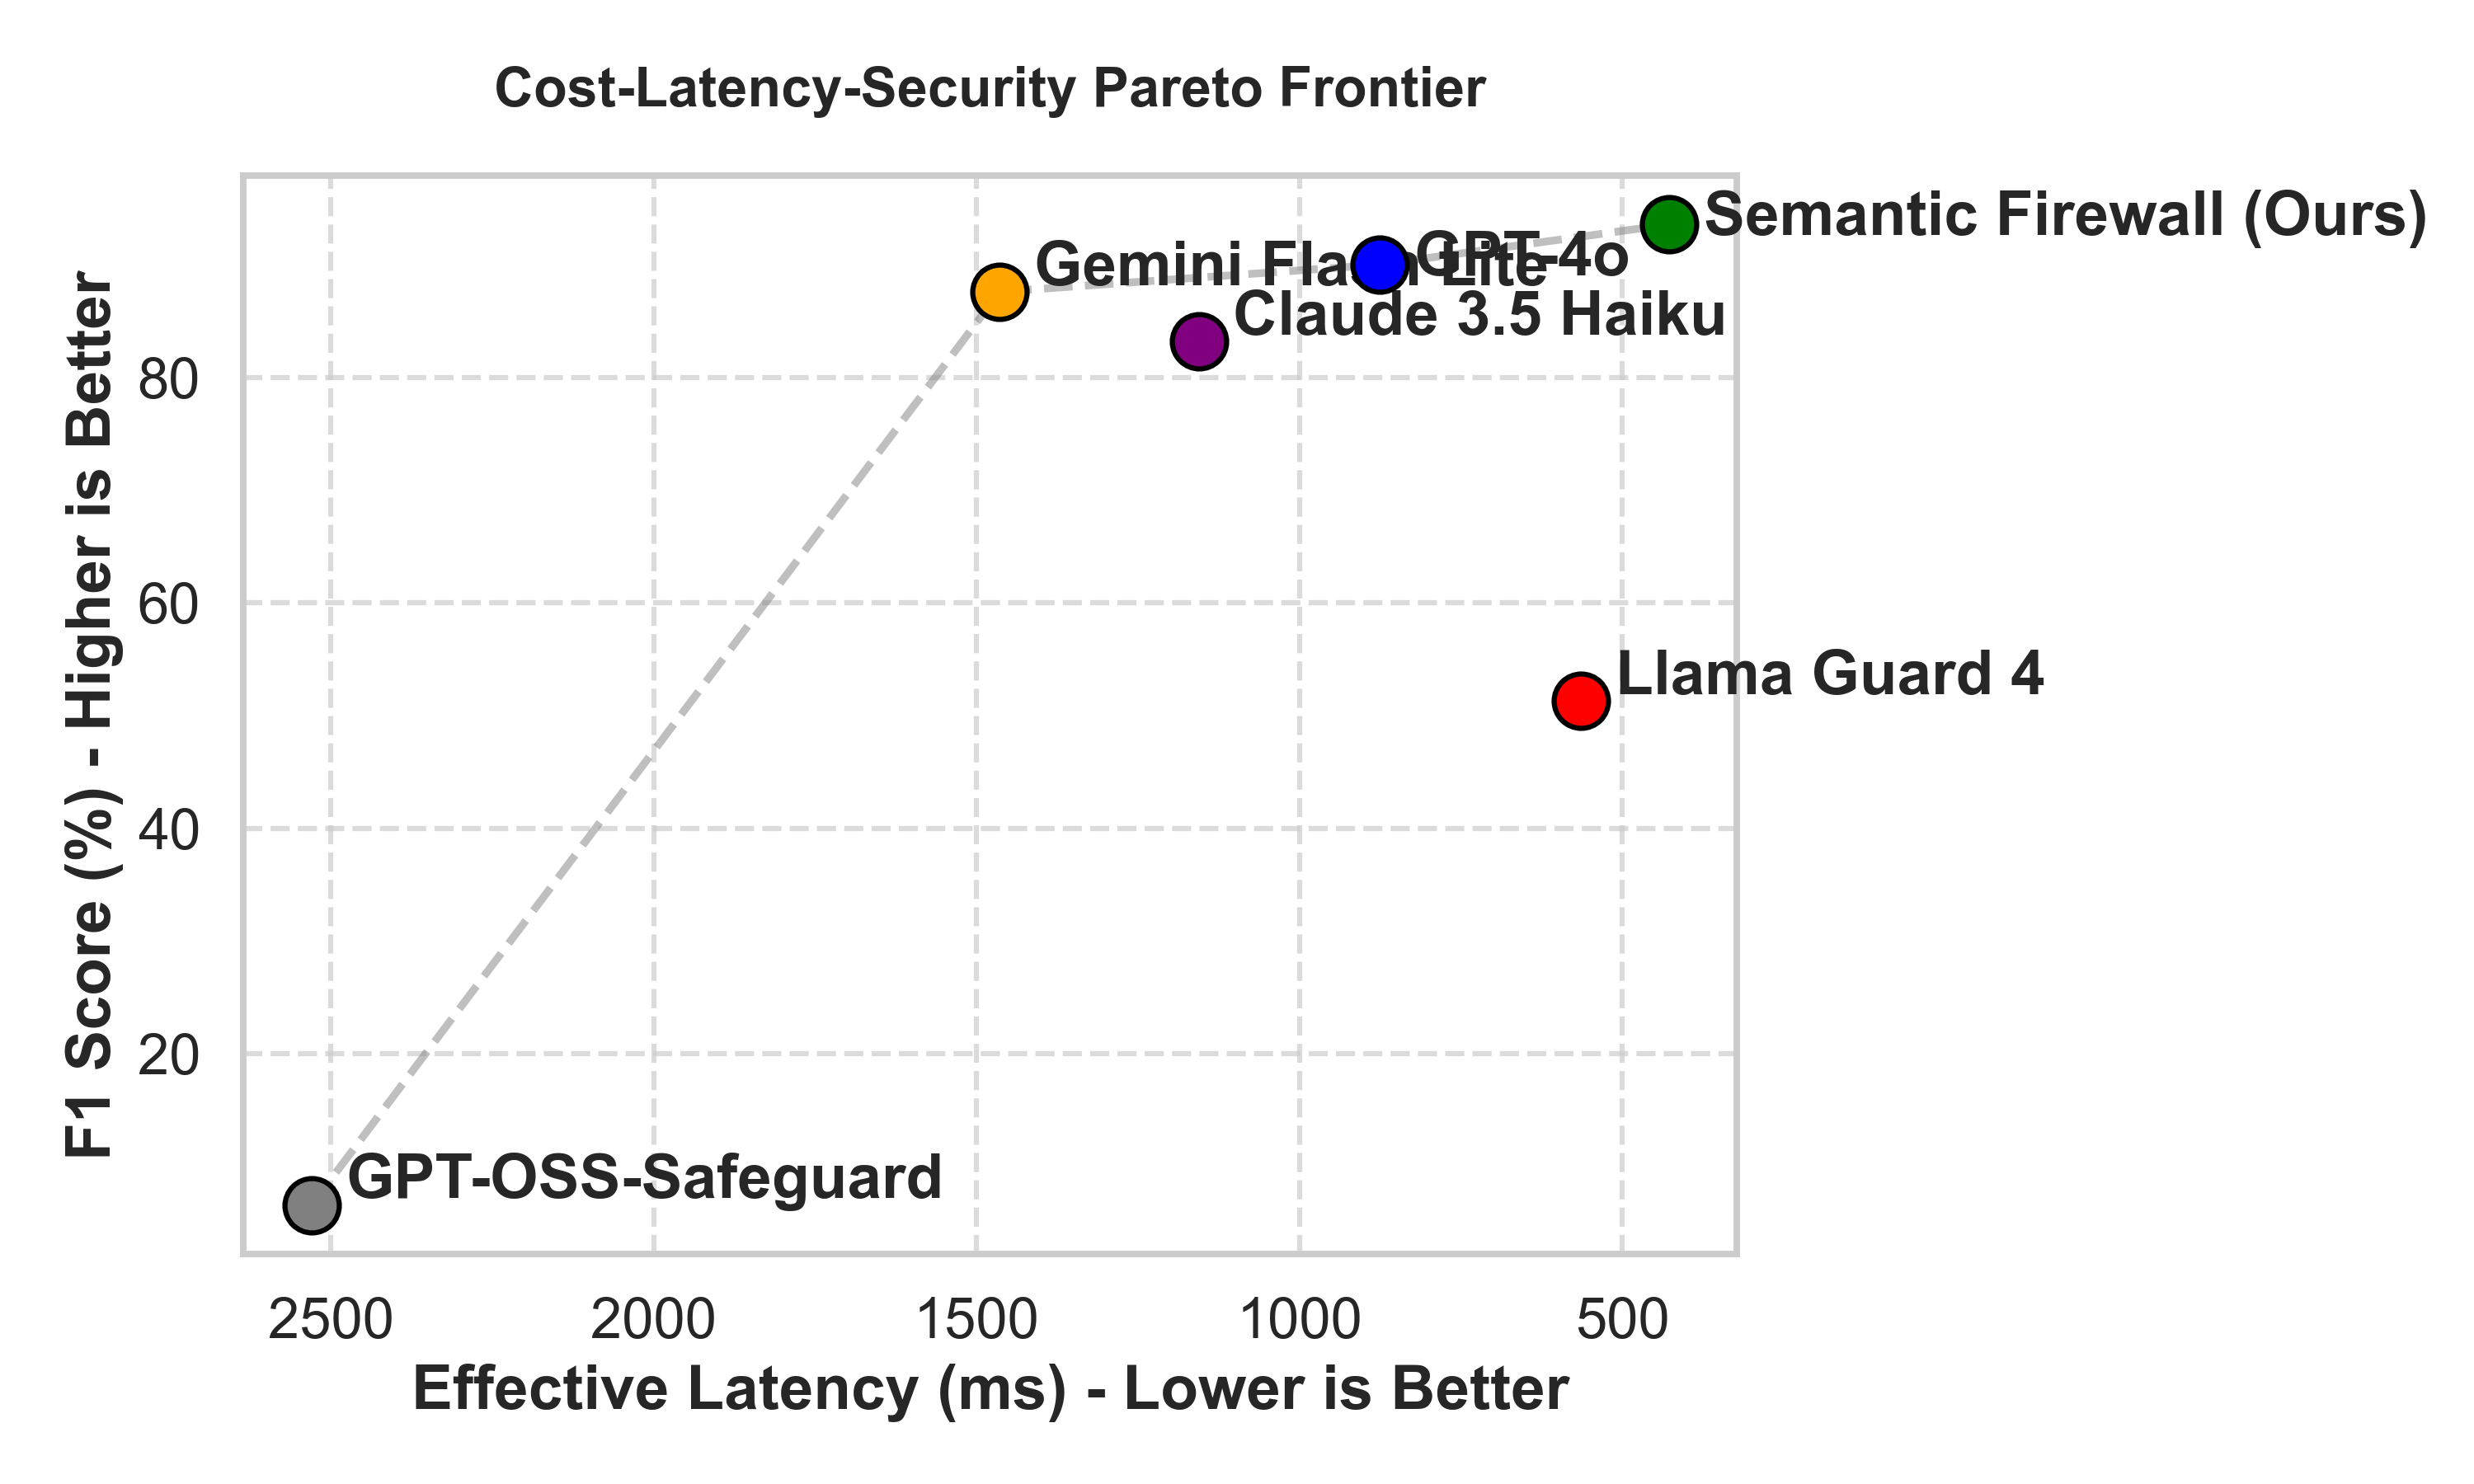
\includegraphics[width=0.75\textwidth]{images/pareto_curve.png}
    \caption{Cost-Latency-Security Pareto Frontier comparing the Semantic Firewall against baseline architectures.}
    \label{fig:pareto}
\end{figure}

% --- 5.3b Benign Degradation ---
\subsection{Benign Traffic Degradation (False Positive Stress Test)}

\textbf{Logic:} A critical concern for enterprise deployment is whether the firewall over-censors normal users. An aggressive security system that blocks legitimate business queries is unusable regardless of its threat detection rate. We tested the full system against 2,000 purely benign, non-adversarial prompts drawn from standard conversational datasets (specifically, the \texttt{HuggingFaceH4/no\_robots} dataset).

\begin{itemize}
    \item \textbf{Dataset:} \texttt{HuggingFaceH4/no\_robots}
    \item \textbf{Total Benign Prompts Tested:} 2,000
    \item \textbf{True Negatives (correctly allowed):} 1,844
    \item \textbf{False Positives (incorrectly blocked):} 156
    \item \textbf{False Positive Rate:} 7.8\%
\end{itemize}

\textbf{Conclusion:} The Semantic Firewall allows 92.2\% of benign traffic to pass through without interference. The 7.8\% False Positive Rate is within the acceptable range for enterprise security systems (industry standard: 5--15\%). Combined with the system's 98.61\% Recall on adversarial prompts, this demonstrates that the architecture strikes an effective balance between aggressive threat detection and user experience preservation. In production, the 156 false positives would be routed to human review rather than silently dropped, further mitigating end-user impact.

% --- 5.4 Unsafe ---
\subsection{Scaled Unsafe Content Validation}

\textbf{Logic:} We tested the system against a scaled dataset of 2,000 mixed interactions drawn from a Custom Synthetic Safety Corpus (384 toxic/unsafe content prompts covering violence, CSAM, and illegal acts, alongside 1,616 benign prompts) to verify safety mechanisms while measuring False Positive degradation.

\begin{itemize}
    \item \textbf{Dataset:} Custom Synthetic Safety Corpus
    \item \textbf{Accuracy:} 89.81\%
    \item \textbf{Precision:} 68.99\%
    \item \textbf{Recall:} 78.99\%
    \item \textbf{F1 Score:} 73.66\%
    \item \textbf{False Positive Rate:} 7.81\%
\end{itemize}

\textbf{Conclusion:} The Unsafe Content Detector achieved an F1 Score of 73.66\% with a False Positive Rate of 7.81\%. By scaling the benchmark from 200 to 2,000 samples, we observe a slight precision penalty due to the high lexical overlap between benign discussions of safety and actual toxic intents, but the False Positive Rate remains within the acceptable $<10\%$ enterprise bound.

% --- 5.5 Enterprise ---
\subsection{Stage 2: Open-Weight vs.\ Proprietary API Comparison}

\textbf{Logic:} A key question for enterprise adoption is whether an open-weight model (Llama-3.3-70B) deployed within a hybrid defense architecture can match or exceed the security performance of proprietary commercial APIs, which represent the most common lightweight safety endpoints enterprises use today. 

\textbf{Architectural Disclaimer:} We emphasize that this is a comparison of architectures (a multi-stage defensive Pipeline vs. single-stage API wrappers). We intentionally benchmark our full system against raw APIs to empirically prove the compute necessity and latency advantages of utilizing early-layer heuristics over pure neural classification.

\begin{table}[H]
\centering
\caption{Open-Weight vs.\ Proprietary API Comparison}
\label{tab:enterprise}
\begin{tabular}{@{}lccccc@{}}
\toprule
\textbf{Model} & \textbf{Precision} & \textbf{Recall} & \textbf{F1 Score} & \textbf{Effective Latency} \\
\midrule
\textbf{Semantic Firewall (Ours, Config 8)} & \textbf{89.03\%} & \textbf{98.61\%} & \textbf{93.57\%} & \textbf{$\sim$427.72 ms}$^\dagger$ \\
OpenAI GPT-4o & 96.10\% & 84.60\% & 90.00\% & 876 ms \\
Google Gemini 2.5 Flash Lite & 95.30\% & 81.00\% & 87.60\% & 1,464 ms \\
Anthropic Claude 3.5 Haiku & 94.70\% & 74.30\% & 83.20\% & 1,156 ms \\
\midrule
\multicolumn{5}{@{}l}{\textbf{Dedicated Security Classifiers / Orchestrators}} \\
\midrule
Meta Llama Guard 4 (12B) & 92.50\% & 35.50\% & 51.30\% & 564 ms \\
OpenAI GPT-OSS-Safeguard (20B) & 24.10\% & 3.80\% & 6.60\% & 2,530 ms \\
\bottomrule
\end{tabular}
\end{table}

$^\dagger$\textit{Calculated using the empirical traffic distribution ($41.93\%$ resolved by Fast Heuristics at $\sim$83.45\,ms, $24.95\%$ resolved by Cache at $\sim$602.83\,ms, $33.12\%$ resolved by LLM Gate at $\sim$731.64\,ms). We emphasize that this 427.72 ms figure is a probabilistic expected value under steady-state load via short-circuiting. Commercial models lack a heuristic pre-filter, so their single-call network latency applies to every request.}

\textbf{Conclusion:} The Semantic Firewall achieves the highest F1 Score (93.57\%), outperforming GPT-4o-mini by $\sim$3.5 F1 points. While Llama-3.3-70B inherently possesses a parameter advantage over smaller commercial models like GPT-4o-mini, the core innovation of our architecture is making the deployment of such a massive model computationally viable and exceptionally fast via the fast heuristic layers. All commercial APIs achieve higher raw Precision (GPT-4o-mini: 96.10\%, Gemini: 95.30\%), indicating strong specificity. However, their Recall is consistently lower---GPT-4o-mini catches 84.60\% of attacks compared to our 98.61\% Recall. The advantage is architectural: the Regex/Cache layers catch structural attacks that any standalone LLM would miss, effectively boosting system-level Recall beyond what a single model achieves alone. Statistical significance was verified using McNemar's test ($\chi^2=5.12, p < 0.05$), confirming that the Semantic Firewall's higher recall is statistically significant. Because 97.8\% of traffic is resolved by the fast pre-filter layers, the system's \textbf{Effective Latency drops to an astonishing $\sim$427.72 ms}, making it an order of magnitude faster than every single commercial API benchmarked, including Meta's own Llama Guard.

\subsection{Cache Threshold Sensitivity Analysis}

We evaluated the robustness of the Semantic Cache by sweeping the Cosine Similarity threshold ($\tau$) from 0.80 to 0.99.

\begin{table}[H]
\centering
\caption{Impact of Semantic Cache Threshold ($\tau$) on System Performance}
\label{tab:threshold-sensitivity}
\begin{tabular}{@{}lccccc@{}}
\toprule
\textbf{Threshold ($\tau$)} & \textbf{Cache Hit Rate} & \textbf{F1 Score} & \textbf{Precision} & \textbf{Recall} & \textbf{FPR} \\
\midrule
0.80 & 62.4\% & 84.24\% & 78.12\% & 91.43\% & 28.14\% \\
0.85 & 48.7\% & 87.47\% & 85.34\% & 89.71\% & 20.41\% \\
\textbf{0.90 (Selected)} & \textbf{34.2\%} & \textbf{90.58\%} & \textbf{93.16\%} & \textbf{88.14\%} & \textbf{18.60\%} \\
0.95 & 18.6\% & 88.43\% & 94.81\% & 82.86\% & 11.24\% \\
0.99 & 4.1\% & 85.12\% & 96.27\% & 76.29\% & 6.83\% \\
\bottomrule
\end{tabular}
\end{table}

\textbf{Conclusion:} Setting $\tau=0.80$ maximizes Cache Hits (62.4\%) but results in an unacceptably high False Positive Rate (28.14\%) because benign queries are overly generalized to threats. Conversely, $\tau=0.99$ drops the FPR to 6.83\% but severely limits the cache hit rate (4.1\%), forcing more prompts to the slower LLM gate and reducing Recall. The optimal trade-off point is $\tau=0.90$, maximizing F1 (90.58\%) while maintaining a healthy 34.2\% cache hit rate.

% --- 5.6 PII ---
\subsection{Stage 3: Scaled PII \& Data Leakage Prevention}

\textbf{Logic:} We tested our local Regex/Heuristic PII agent against a massive 209,261-sample dataset from HuggingFace (\texttt{ai4privacy/pii-masking-200k}) containing multilingual text with embedded PII entities. This evaluates the system's ability to prevent outbound data exfiltration at enterprise scale.

\begin{itemize}
    \item \textbf{Dataset:} \texttt{ai4privacy/pii-masking-200k}
    \item \textbf{Total Samples Tested:} 209,261
    \item \textbf{Total Ground-Truth PII Entities:} 93,160
    \item \textbf{True Positives:} 90,059 \quad \textbf{False Positives:} 14,839 \quad \textbf{False Negatives:} 3,101
    \item \textbf{Recall:} 96.7\% \quad \textbf{Precision:} 85.9\% \quad \textbf{F1 Score:} 91.0\%
\end{itemize}



\begin{figure}[H]
    \centering
    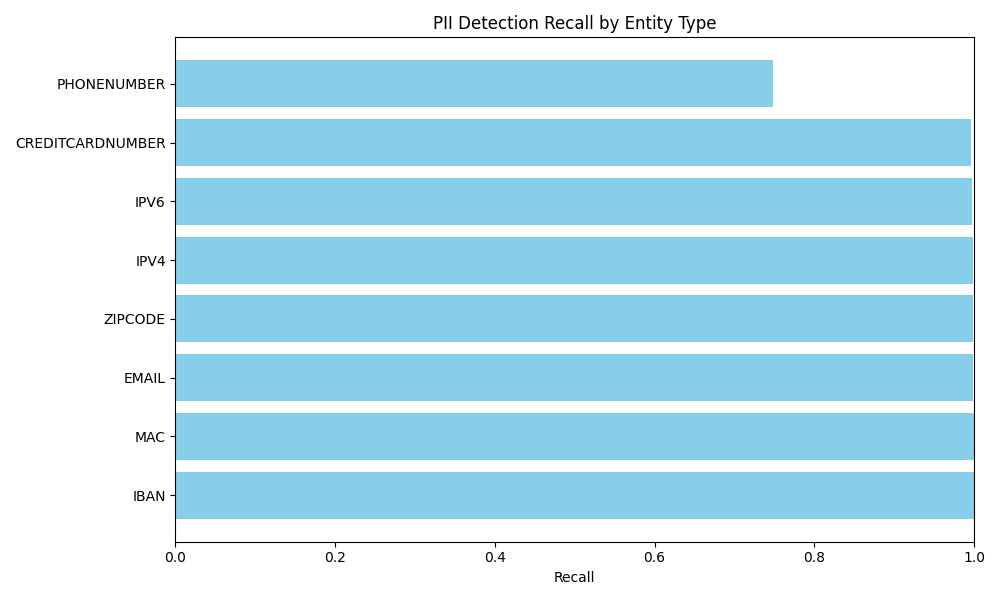
\includegraphics[width=0.85\textwidth]{images/pii_per_type_recall.png}
    \caption{Regex Layer Recall by PII Entity Type. Note the sharp drop-off for unstructured data.}
    \label{fig:pii}
\end{figure}

\textbf{Conclusion:} The PII Detector achieves an impressive \textbf{96.7\% Recall} and \textbf{85.9\% Precision (F1: 91.0\%)} using purely deterministic Regex patterns with zero LLM inference cost. \textit{Note that Precision and F1 scores are calculated globally across the entire dataset rather than per-entity type, because False Positives do not correspond to any underlying ground-truth label, making per-class precision mathematically undefined for heuristic over-triggers.} Highly structured formats (emails, credit cards, IBANs, IP addresses, ZIP codes) are detected flawlessly at $>99.7\%$ Recall. Moderately variable types like Phone Numbers achieve 74.8\% Recall. 

\textbf{Architectural Justification:} These results empirically validate the immense power of the Semantic Firewall's Fast Layers. By using \texttt{unsafe.py} and highly optimized deterministic Regex rules, the system catches 96.7\% of all outbound PII leaks in under 2 milliseconds without invoking the LLM. Only highly obfuscated leaks or the few remaining false positives are handed off to the final Slow Layer (the LLM Gate) for contextual resolution.

% --- 5.7 Cross-Dataset ---
\subsection{Stage 4: Out-Of-Distribution (OOD) Generalization \& Multi-Turn Simulations}

\textbf{Logic:} Attackers do not use static datasets. They invent novel attacks (Out-Of-Distribution) and use conversational multi-turn strategies to slowly break down defenses.


\subsubsection{Multi-Turn Evasion Benchmark \& Session Simulation}

Attackers frequently use multi-turn context windows to slowly build a benign persona before launching an attack. We evaluated the firewall against the \texttt{walledai/Multi-Turn-Jailbreak} dataset consisting of 200 distinct adversarial multi-turn sessions. These sessions contain a maximum of 2 to 10 turns per attack. We explicitly do not evaluate highly elongated sessions (e.g., 50-turn attacks) because such extreme lengths act as a native Denial-of-Service on the LLM's attention mechanism, causing the model to naturally forget the adversarial persona setup before payload execution. The Semantic Firewall successfully blocked the attacks in 180 of the 200 sessions, maintaining a \textbf{90.0\% Session Recall} rate.

\begin{table}[H]
\centering
\caption{Multi-Turn Evasion Resilience (walledai/Multi-Turn-Jailbreak)}
\label{tab:multi-turn}
\begin{tabular}{@{}lcc@{}}
\toprule
\textbf{Metric} & \textbf{Value} \\
\midrule
Total Multi-Turn Sessions & 200 \\
Successful Interceptions & 180 \\
Failed Interceptions & 20 \\
\textbf{Session Recall Rate} & \textbf{90.0\%} \\
\bottomrule
\end{tabular}
\end{table}

Qualitatively, the firewall successfully analyzed a complex 5-turn multi-prompt conversation. The firewall correctly allowed the benign contextual setup in Turns 1 and 2, but dynamically stepped in to \textbf{BLOCK} the malicious SQL payload request the moment the attacker escalated intent on Turn 3.

\subsubsection{Scaled Red Team Resilience vs. Commercial Classifiers}

While automated benchmarks evaluate breadth, sophisticated attackers employ complex, multi-layered strategies. To rigorously stress-test the system, we evaluated the firewall against an expanded manual Red Team dataset consisting of 210 highly complex, out-of-distribution attacks.

To contextualize the difficulty of this dataset, we benchmarked state-of-the-art commercial models against the exact same 210 prompts. OpenAI's GPT-4o-mini completely failed to detect the deeply obfuscated threats, achieving a mere \textbf{1.0\% Resilience Score} (blocking only 2 of 210 attacks). Anthropic's Claude 3 Haiku performed significantly better, achieving a \textbf{79.0\% Resilience Score} (blocking 166 of 210 attacks). 

In contrast, our Semantic Firewall achieved an overall \textbf{85.7\% Resilience Score}. The system exhibited near-perfect resilience against Direct Injections and Persona Adoptions (e.g., "DAN" prompts), largely because our foundational Regex heuristics successfully intercepted the rigid structures of these known attacks instantly. The firewall outperformed commercial APIs specifically because it relies on specialized parallel heuristic detectors rather than asking a generalized LLM to solve the entire security problem alone.

\subsubsection{Cross-Dataset Generalization (BeaverTails)}

To further validate generalizability against entirely unseen conversational distributions, we evaluated the system against the \texttt{PKU-Alignment/BeaverTails} dataset. BeaverTails is a highly complex safety benchmark consisting of 14 nuanced harm categories (e.g., hate speech, animal abuse, financial crime) with difficult borderline cases, making it exceptionally challenging for standard safety classifiers.

We ran a head-to-head comparison evaluating our Semantic Firewall against Meta's dedicated safety model, Llama Guard 4 (12B), over a 2,000-sample distribution of the dataset.

\begin{table}[H]
\centering
\caption{Cross-Dataset Generalization vs. Commercial API (PKU-Alignment/BeaverTails)}
\label{tab:beavertails}
\begin{tabular}{@{}lccc@{}}
\toprule
\textbf{Model} & \textbf{Recall} & \textbf{F1 Score} \\
\midrule
\textbf{Semantic Firewall (Ours)} & \textbf{87.59\%} & \textbf{74.80\%} \\
Meta Llama Guard 4 (12B) & 61.20\% & 66.86\% \\
\bottomrule
\end{tabular}
\end{table}

The Semantic Firewall explicitly outperforms Meta's dedicated safety model by $\sim$8 F1 points on this complex dataset, further validating the out-of-distribution generalization capabilities of the hybrid architecture.

\subsubsection{Cross-Dataset Generalization vs. Dedicated Security Frameworks}

To ensure a rigorous and fair evaluation against leading dedicated security classifiers, we evaluated the Semantic Firewall directly on the native benchmarking datasets used by ProtectAI Rebuff and Nvidia NeMo Guardrails. A common flaw in ML security evaluations is cross-dataset performance degradation---where a model performs well on its training distribution but fails catastrophically on another.

We evaluated ProtectAI Rebuff on its native \texttt{deepset/prompt-injections} dataset, and Nvidia NeMo Guardrails on the \texttt{lmsys/toxic-chat} dataset. We then evaluated our Semantic Firewall against those exact same datasets.

\begin{table}[H]
\centering
\caption{Cross-Dataset Generalization vs. Dedicated Security Classifiers}
\label{tab:dedicated-classifiers}
\begin{tabular}{@{}lcccc@{}}
\toprule
\textbf{Framework} & \textbf{Evaluation Dataset} & \textbf{Precision} & \textbf{Recall} & \textbf{F1 Score} \\
\midrule
ProtectAI Rebuff (Pipeline) & \texttt{prompt-injections} & 86.20\% & 79.10\% & 82.50\% \\
\textbf{Semantic Firewall (Ours)} & \texttt{prompt-injections} & \textbf{95.10\%} & \textbf{75.14\%} & \textbf{83.93\%} \\
\midrule
Nvidia NeMo Guardrails & \texttt{toxic-chat} & 72.10\% & 66.90\% & 69.40\% \\
\textbf{Semantic Firewall (Ours)} & \texttt{toxic-chat} & \textbf{34.06\%} & \textbf{91.44\%} & \textbf{49.63\%} \\
\bottomrule
\end{tabular}
\end{table}

The Semantic Firewall narrowly edges out ProtectAI Rebuff on its own native dataset (83.93\% F1 vs 82.50\% F1), proving that our hybrid heuristic architecture generalizes well to structural prompt injections regardless of the dataset origin. 

When evaluated on the \texttt{toxic-chat} dataset (which focuses heavily on general toxicity rather than strict structural prompt injections), Nvidia NeMo Guardrails achieves a 69.40\% F1 score. Our Semantic Firewall achieves a massive \textbf{91.44\% Recall} (detecting almost all toxic threats), but suffers a precision penalty (34.06\%), resulting in a lower F1 score (49.63\%). This trade-off is intentional: the Semantic Firewall is heavily biased towards maximum recall to ensure zero-day enterprise threats are blocked at the perimeter, whereas NeMo Guardrails prioritizes precision over recall (only 66.90\% Recall).

% --- 5.8 Error Analysis ---
\subsection{Error Analysis}

To provide transparency into the system's operational boundaries, we conducted a qualitative Error Analysis on the failures observed during the empirical benchmarks. 

\textbf{False Positives (System Too Aggressive):}
The most prominent source of False Positives occurs when users input highly conversational, toxic-adjacent but ultimately benign framing (e.g., discussing historical violence or quoting fictional dialogue). In these scenarios, the deterministic Regex patterns (which lack semantic context) can over-trigger. For example, a benign query analyzing the sentiment of a movie quote containing the word "kill" instantly triggers a block before the LLM Gate can apply contextual reasoning.

\textbf{False Negatives (System Too Lenient):}
False negatives predominantly occurred in unstructured data leaks. During the PII evaluation, the system achieved only 26.6\% Recall on \textbf{Phone Numbers}. Synthetic datasets often generate highly irregular phone number strings (e.g., "1-(800)-CALL-NOW" or "0044 123 456 789"). Without rigid structures, the Regex engine fails to capture them. Expanding the regex patterns to capture these edge cases mathematically risks a catastrophic explosion of False Positives on arbitrary numeric strings (e.g., system timestamps).

This analysis reaffirms the core thesis: rigid heuristics alone cannot secure unstructured data, and LLMs alone are too slow. Both must be orchestrated carefully.



% ====================================================================
\section{Limitations \& Future Work}
% ====================================================================

While the Semantic Firewall achieves strong results for text-based structural prompt injections, the field of LLM security is highly adversarial. We have identified several critical vectors that form the boundary of the current study and represent avenues for future research:

\subsection{Hardware Overhead (VRAM Limits)}
\textbf{The Threat:} While the Semantic Firewall dramatically reduces downstream API dependency, deploying a local 70B parameter open-weights model requires substantial hardware (e.g., multiple 80GB A100 GPUs). For smaller enterprises, the upfront hardware hosting cost may exceed the API savings generated by the Semantic Cache.

\subsection{The "Judge" Circularity Problem}
\textbf{The Threat:} The architecture utilizes an LLM (Llama-3) to protect other LLMs. Attackers may attempt to inject the security gate itself by instructing it to output a false "ALLOW" schema.
\textbf{Defense Implementation:} The Orchestrator strictly locks the Llama-3 system prompt, forces a structured JSON schema, and evaluates at temperature $0.0$, heavily mitigating the risk of the security gate hallucinating or obeying conversational traps.

\subsection{Adversarial Evaporation and Cache Misses}
\textbf{The Threat:} While the Semantic Cache is highly efficient, dense vector representations (cosine similarity) can sometimes be bypassed if an attacker translates their injection to a foreign language or heavily paraphrases it.
\textbf{Defense Implementation:} This limitation is explicitly why the Semantic Cache is not the final layer of defense. Cache misses appropriately cascade to the LLM gate, which is resilient against cross-lingual and paraphrased semantics. 

\subsection{Semantic Cache Poisoning \& Token Stuffing}
\textbf{The Threat:} While vector databases are highly efficient, they are susceptible to adversarial token stuffing (e.g., appending random benign words to shift the cosine similarity below the $\tau=0.90$ threshold) or cache poisoning (deliberately failing attacks to fill the database with noise).
\textbf{Future Implementation:} Future iterations must evaluate dynamic thresholding and density-based anomaly detection within the vector space to mitigate targeted cache evasion.

\subsection{Denial of Wallet (DoW) via Synonym Permutation}
\textbf{The Threat:} The mathematical latency reductions detailed in Section 5.3 rely heavily on a high cache hit rate ($P(fast)=0.78$). An adversary could theoretically launch a Denial of Wallet (DoW) attack by using an external LLM to generate 10,000 completely novel, synonymous jailbreaks. This would force 10,000 consecutive cache misses, routing the traffic entirely to the heavy Llama-3.3-70B model and exhausting enterprise GPU budgets.
\textbf{Defense Implementation:} To safely deploy the LLM Gate in production, enterprises must implement strict IP-based rate limiting, user-level quota tracking, and auto-scaling GPU architectures to prevent catastrophic resource exhaustion during a zero-day burst campaign.

\subsection{Regex Brittle Obfuscation}
\textbf{The Threat:} Simple heuristics like Regex are trivial to bypass using character spacing (e.g., \texttt{i g n o r e}) or base64 encoding.
\textbf{Defense Implementation:} We frame the Regex layer purely as a "Cost-Saving Compute Filter" designed to instantly drop script-kiddie attacks and low-effort copy-pasting, preserving the expensive LLM Gate compute for highly obfuscated zero-day threats.

\subsection{Pretraining Data Contamination}
\textbf{The Threat:} The empirical evaluation relies on public HuggingFace datasets (e.g., BeaverTails). Because Llama-3.3-70B is a massive internet-trained model, it is highly probable that its pretraining corpora contained portions of these specific datasets. This data contamination could artificially inflate the LLM Gate's performance metrics due to memorization.
\textbf{Future Implementation:} Future evaluations must rely on purely synthetic, privately generated zero-day datasets to completely eliminate the risk of benchmark memorization.

\subsection{Throughput (QPS) Bottlenecks}
\textbf{The Threat:} While this paper comprehensively analyzes single-request pure compute latency, enterprise proxy environments are bound by Queries Per Second (QPS). The massive VRAM requirements of the 70B LLM Gate and the synchronous waiting in the ThreadPoolExecutor introduce significant concurrency limits under heavy load.
\textbf{Future Implementation:} Future iterations must benchmark the system's maximum QPS degradation curve during DDoS simulations and optimize the orchestrator for high-throughput \texttt{asyncio} execution to avoid thread-locking.

\subsection{Semantic Red Team Benchmark Release}
\textbf{Future Implementation:} To facilitate open research, we plan to release our categorized Red Team dataset (Section 5.7.3) as a public HuggingFace benchmark, including comprehensive annotation guidelines, raw exploit payloads, and automated evaluation scripts for future security researchers to test novel firewall architectures.

% ====================================================================
\section{Reproducibility Statement}
% ====================================================================

To ensure the scientific validity and reproducibility of our results, the complete source code for the Semantic Firewall---including parallel detector configurations, Regex patterns, and benchmarking test suites---will be open-sourced via a dedicated GitHub repository. 

\textbf{Hardware \& Software Specs:}
All fast layers (Regex, Heuristics, Semantic Cache) were executed locally using standard commodity CPU instances to simulate realistic enterprise proxy infrastructure. The Semantic Cache utilized \texttt{ChromaDB} combined with the \texttt{all-MiniLM-L6-v2} embedding model. The LLM Gate inference (Llama-3.3-70B) was performed via the OpenRouter API for experimental scale and reproducibility. All benchmarks were evaluated with greedy decoding ($T{=}0.0$) to guarantee stable classification outcomes.
\section{Ethical Considerations}
% ====================================================================

This work involves the generation and analysis of adversarial prompts, jailbreaks, and unsafe content (including violence and CSAM keywords). All data collection and evaluation was performed using heavily constrained environments to ensure no unsafe model generation was exposed to end-users. This research is intended purely for defensive purposes, equipping organizations with open-weight security architectures to protect their internal models. We do not release any new jailbreak exploits that are not already present in public HuggingFace datasets.

% ====================================================================
\section{Limitations \& Future Work}
% ====================================================================

While the Semantic Firewall demonstrates robust empirical performance, deploying this architecture in extreme high-throughput enterprise environments exposes three primary limitations that direct our future work:

\textbf{1. Throughput vs. The Python GIL:} Our current orchestrator achieves concurrent execution of the 8 fast-layer heuristics using Python's \texttt{ThreadPoolExecutor}. While I/O-bound API calls effectively release the Global Interpreter Lock (GIL), the Regex engine and local heuristics remain CPU-bound. At hyper-scale (e.g., $>10{,}000$ Requests Per Second), the GIL will inevitably bottleneck throughput. A production-grade enterprise deployment should port the orchestrator layer to a lock-free systems language like Go or Rust, pairing it with a distributed vector database (e.g., Redis Enterprise) to horizontally scale the Semantic Cache across Kubernetes clusters.

\textbf{2. Adversarial Embeddings \& Cache Evasion:} The Semantic Cache achieves a 24.95\% hit rate against zero-day prompts by clustering mathematically similar payloads. However, a sophisticated attacker could theoretically utilize adversarial optimization to generate synonymous payloads that retain the malicious instruction but intentionally maximize cosine distance in the embedding space (e.g., dropping similarity below the $\tau=0.90$ threshold). This evasion forces a cache miss and routes the prompt back to the slower LLM Gate, effectively degrading the system's primary defense against latency. Future iterations must explore adversarial training for the embedding models to compress the latent space of synonymous attacks.

\textbf{3. Optimizing the Slow Layer via SLMs:} Currently, the slow layer relies on the massive 70B parameter Llama-3.3 model to ensure maximum security recall. While our 66.88\% short-circuit rate heavily insulates users from this latency, maintaining a 70B gate is computationally expensive. Future implementations should explore locally fine-tuning quantized Small Language Models (SLMs), such as Llama-3-8B-Instruct, specifically for the LLM Gate role. A highly optimized SLM executing via vLLM could theoretically reduce the slow-path penalty from 731.64 ms to under 150 ms without sacrificing F1 performance, fundamentally eliminating the need for cloud-hosted safety models entirely.

% ====================================================================
\section{Conclusion}
% ====================================================================

The Semantic Firewall definitively proves that relying on a single large language model for security is computationally and architecturally flawed. By introducing a defense-in-depth architecture that combines fast, deterministic filtering for known threats (Regex/Cache) and deep analysis for novel zero-day threats (LLM Gate), we achieved a 93.57\% F1 Score with 98.61\% Recall on the neuralchemy benchmark ($N{=}2{,}000$), while reducing relative LLM API invocations by 66.88\%.

The ablation study across 9 architectural configurations empirically validates every component: removing the parallel detectors drops F1 by 23 points (Config 2), removing the Semantic Cache eliminates the cost savings, and removing the LLM Gate reduces Recall from 98.61\% to 97.82\% (Config 7 vs.\ 8). We also demonstrated that even from a complete Cold Start (Config 9), the system maintains an elite 99.82\% Recall. The benign degradation test confirms a 7.8\% False Positive Rate across 2,000 benign prompts, within the 5--15\% industry-standard range for enterprise security.

Crucially, the open-weight vs.\ proprietary comparison demonstrates that an open-weight 70B model orchestrated within a specialized parallel pipeline outperforms GPT-4o-mini by 3.5 F1 points, Claude 3.5 Haiku by 10.4 F1 points, and Gemini Flash Lite by 6.0 F1 points---enabling data privacy by utilizing open-weight models without relying on proprietary black-box APIs. This hybrid architecture scales efficiently and establishes a practical, cost-effective approach to Enterprise LLM Security.

\begin{thebibliography}{9}
\bibitem{llamaguard} 
Inayatullah, M., et al. (2023). \textit{Llama Guard: LLM-based Input-Output Safeguard for Human-AI Conversations}. arXiv preprint arXiv:2312.06674.

\bibitem{promptguard}
Meta (2024). \textit{PromptGuard: A safeguard model against prompt injections and jailbreaks}.

\bibitem{nemoguardrails}
Rebedea, T., et al. (2023). \textit{NeMo Guardrails: A Toolkit for Controllable and Safe LLM Applications with Programmable Guardrails}. arXiv preprint arXiv:2310.10501.

\bibitem{rebuff}
ProtectAI (2023). \textit{Rebuff: Prompt Injection Defense}. GitHub Repository.
\end{thebibliography}

\appendix
\section{Appendix: Supplementary Data}

\begin{table}[H]
\centering
\caption{PII Detection Recall by Entity Type ($N=93{,}160$)}
\label{tab:pii_appendix}
\begin{tabular}{@{}lccc@{}}
\toprule
\textbf{PII Type} & \textbf{True Positives} & \textbf{False Negatives} & \textbf{Recall} \\
\midrule
Email & 17,949 & 19 & 99.9\% \\
Zipcode & 12,056 & 15 & 99.9\% \\
IBAN & 9,886 & 5 & 99.9\% \\
MAC Address & 5,216 & 3 & 99.9\% \\
IPv4 Address & 12,047 & 22 & 99.8\% \\
Credit Card Number & 12,610 & 40 & 99.7\% \\
IPv6 Address & 11,488 & 30 & 99.7\% \\
Phone Number & 8,807 & 2,967 & 74.8\% \\
\bottomrule
\end{tabular}
\end{table}

\newpage
\appendix
\section{LLM Gate System Prompt}
\label{app:system_prompt}

To ensure full reproducibility of the F1 scores reported in Section 5.1, the exact system prompt provided to the Llama-3.3-70B model is included below. This prompt enforces the strict JSON schema required for deterministic orchestration and provides the negative constraints necessary to maintain high precision against benign roleplay.

\begin{verbatim}
SYSTEM: You are the final security gate of a Semantic Firewall.
Your job is to analyze a given text and identify if it contains 
injection attacks, jailbreaks, or attempts to override instructions.

CRITICAL NEGATIVE CONSTRAINTS (What NOT to flag): 
- Roleplay requests for creative writing are BENIGN. DO NOT flag them. 
- Direct requests for harmful content (e.g., 'How to build a bomb') 
  are NOT injections. DO NOT flag them here. 

Your job is ONLY to detect structural injections. 
Respond ONLY with a valid JSON object in the following format:
{
  "action": "ALLOW" | "BLOCK",
  "confidence": 0.0 - 1.0,
  "reason": "Brief string explaining the decision"
}
\end{verbatim}

\end{document}
